
\begin{frame}{Dataset A}
    \begin{columns}[c]        
        % Colonna Sinistra: Testo
        \begin{column}{0.48\textwidth}
        
        Divisione dei dati: Training set \ \ Test set
        
        \vspace{0.7em}
        
        Verifica dei risultati soap
        
        \vspace{0.5em}
        
        {
      		\centering 
        	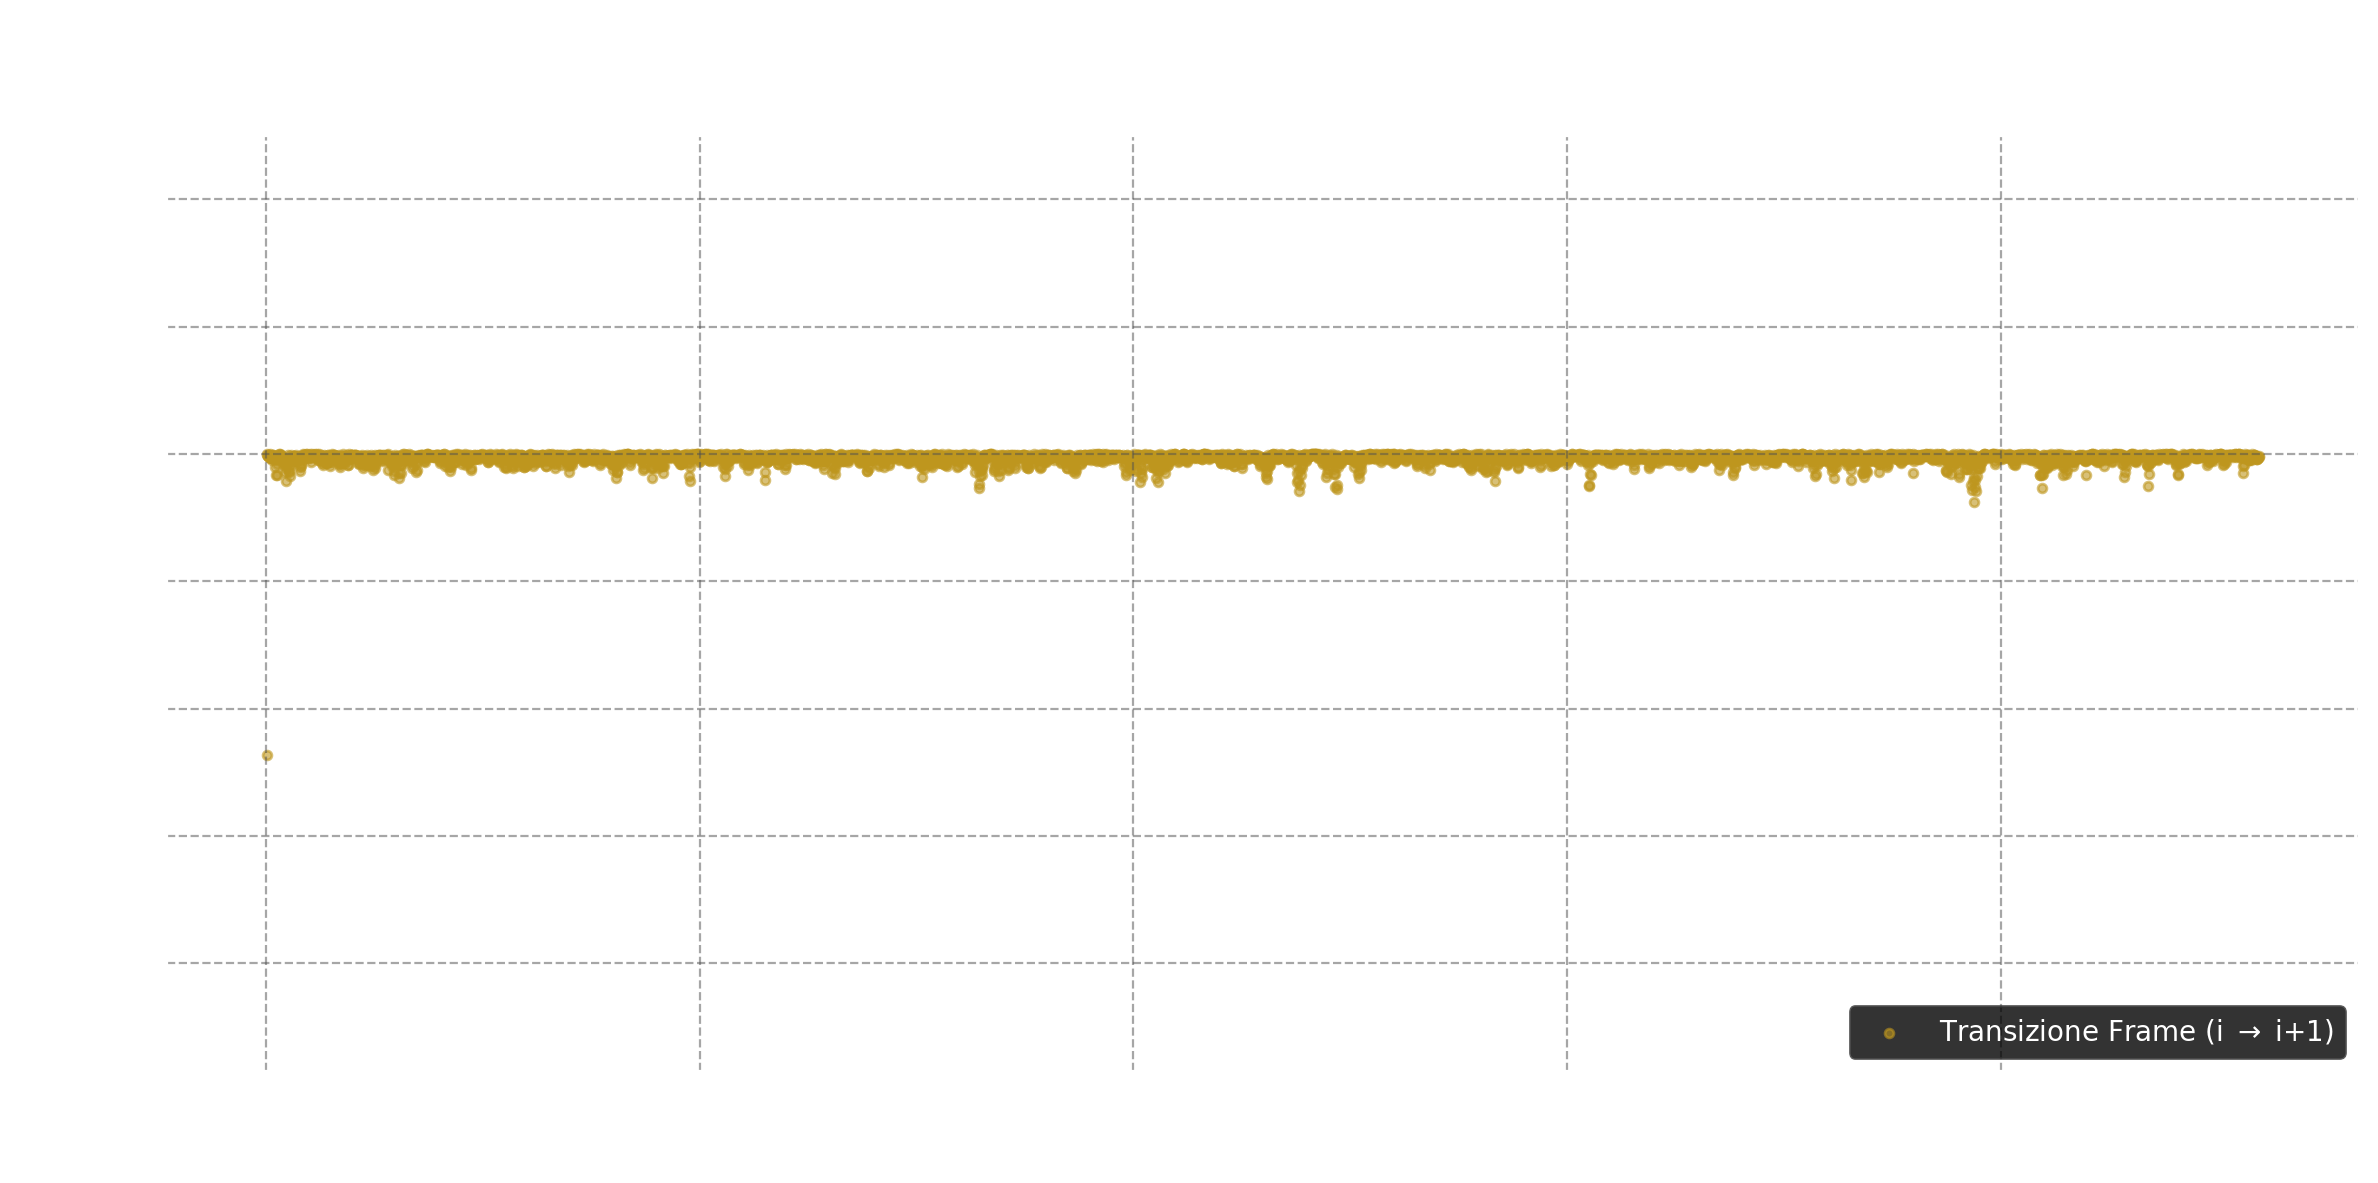
\includegraphics[scale=0.23]{./invnobg/kernel.png}
        }
        
        \end{column}
        % Colonna Destra: Due immagini incolonnate
        \begin{column}{0.48\textwidth}
        
            \begin{flushright}
            	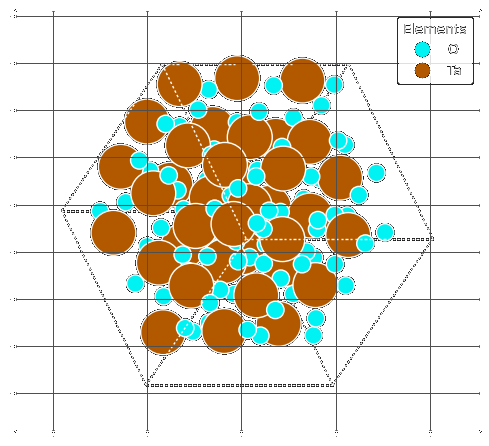
\includegraphics[scale=0.3]{./invnobg/cristallo-from-ase-frame-0-dataset-a.png}
            \end{flushright}
            \begin{flushright}
            	\small{Frame del dataset A \\ generato con matplotlib}
            \end{flushright}
            
            
        \end{column}
    \end{columns}
\end{frame}


\subsection{Energie e forze} %---------------------------------------------------------------------------------------------------------------------------


\begin{frame}{Verifica delle energie e delle forze}
    \begin{columns}[c]        
        % Colonna Sinistra: Testo
        \begin{column}{0.46\textwidth}
 
            \centering
            
            Training set 
            \vspace{6pt}
            
            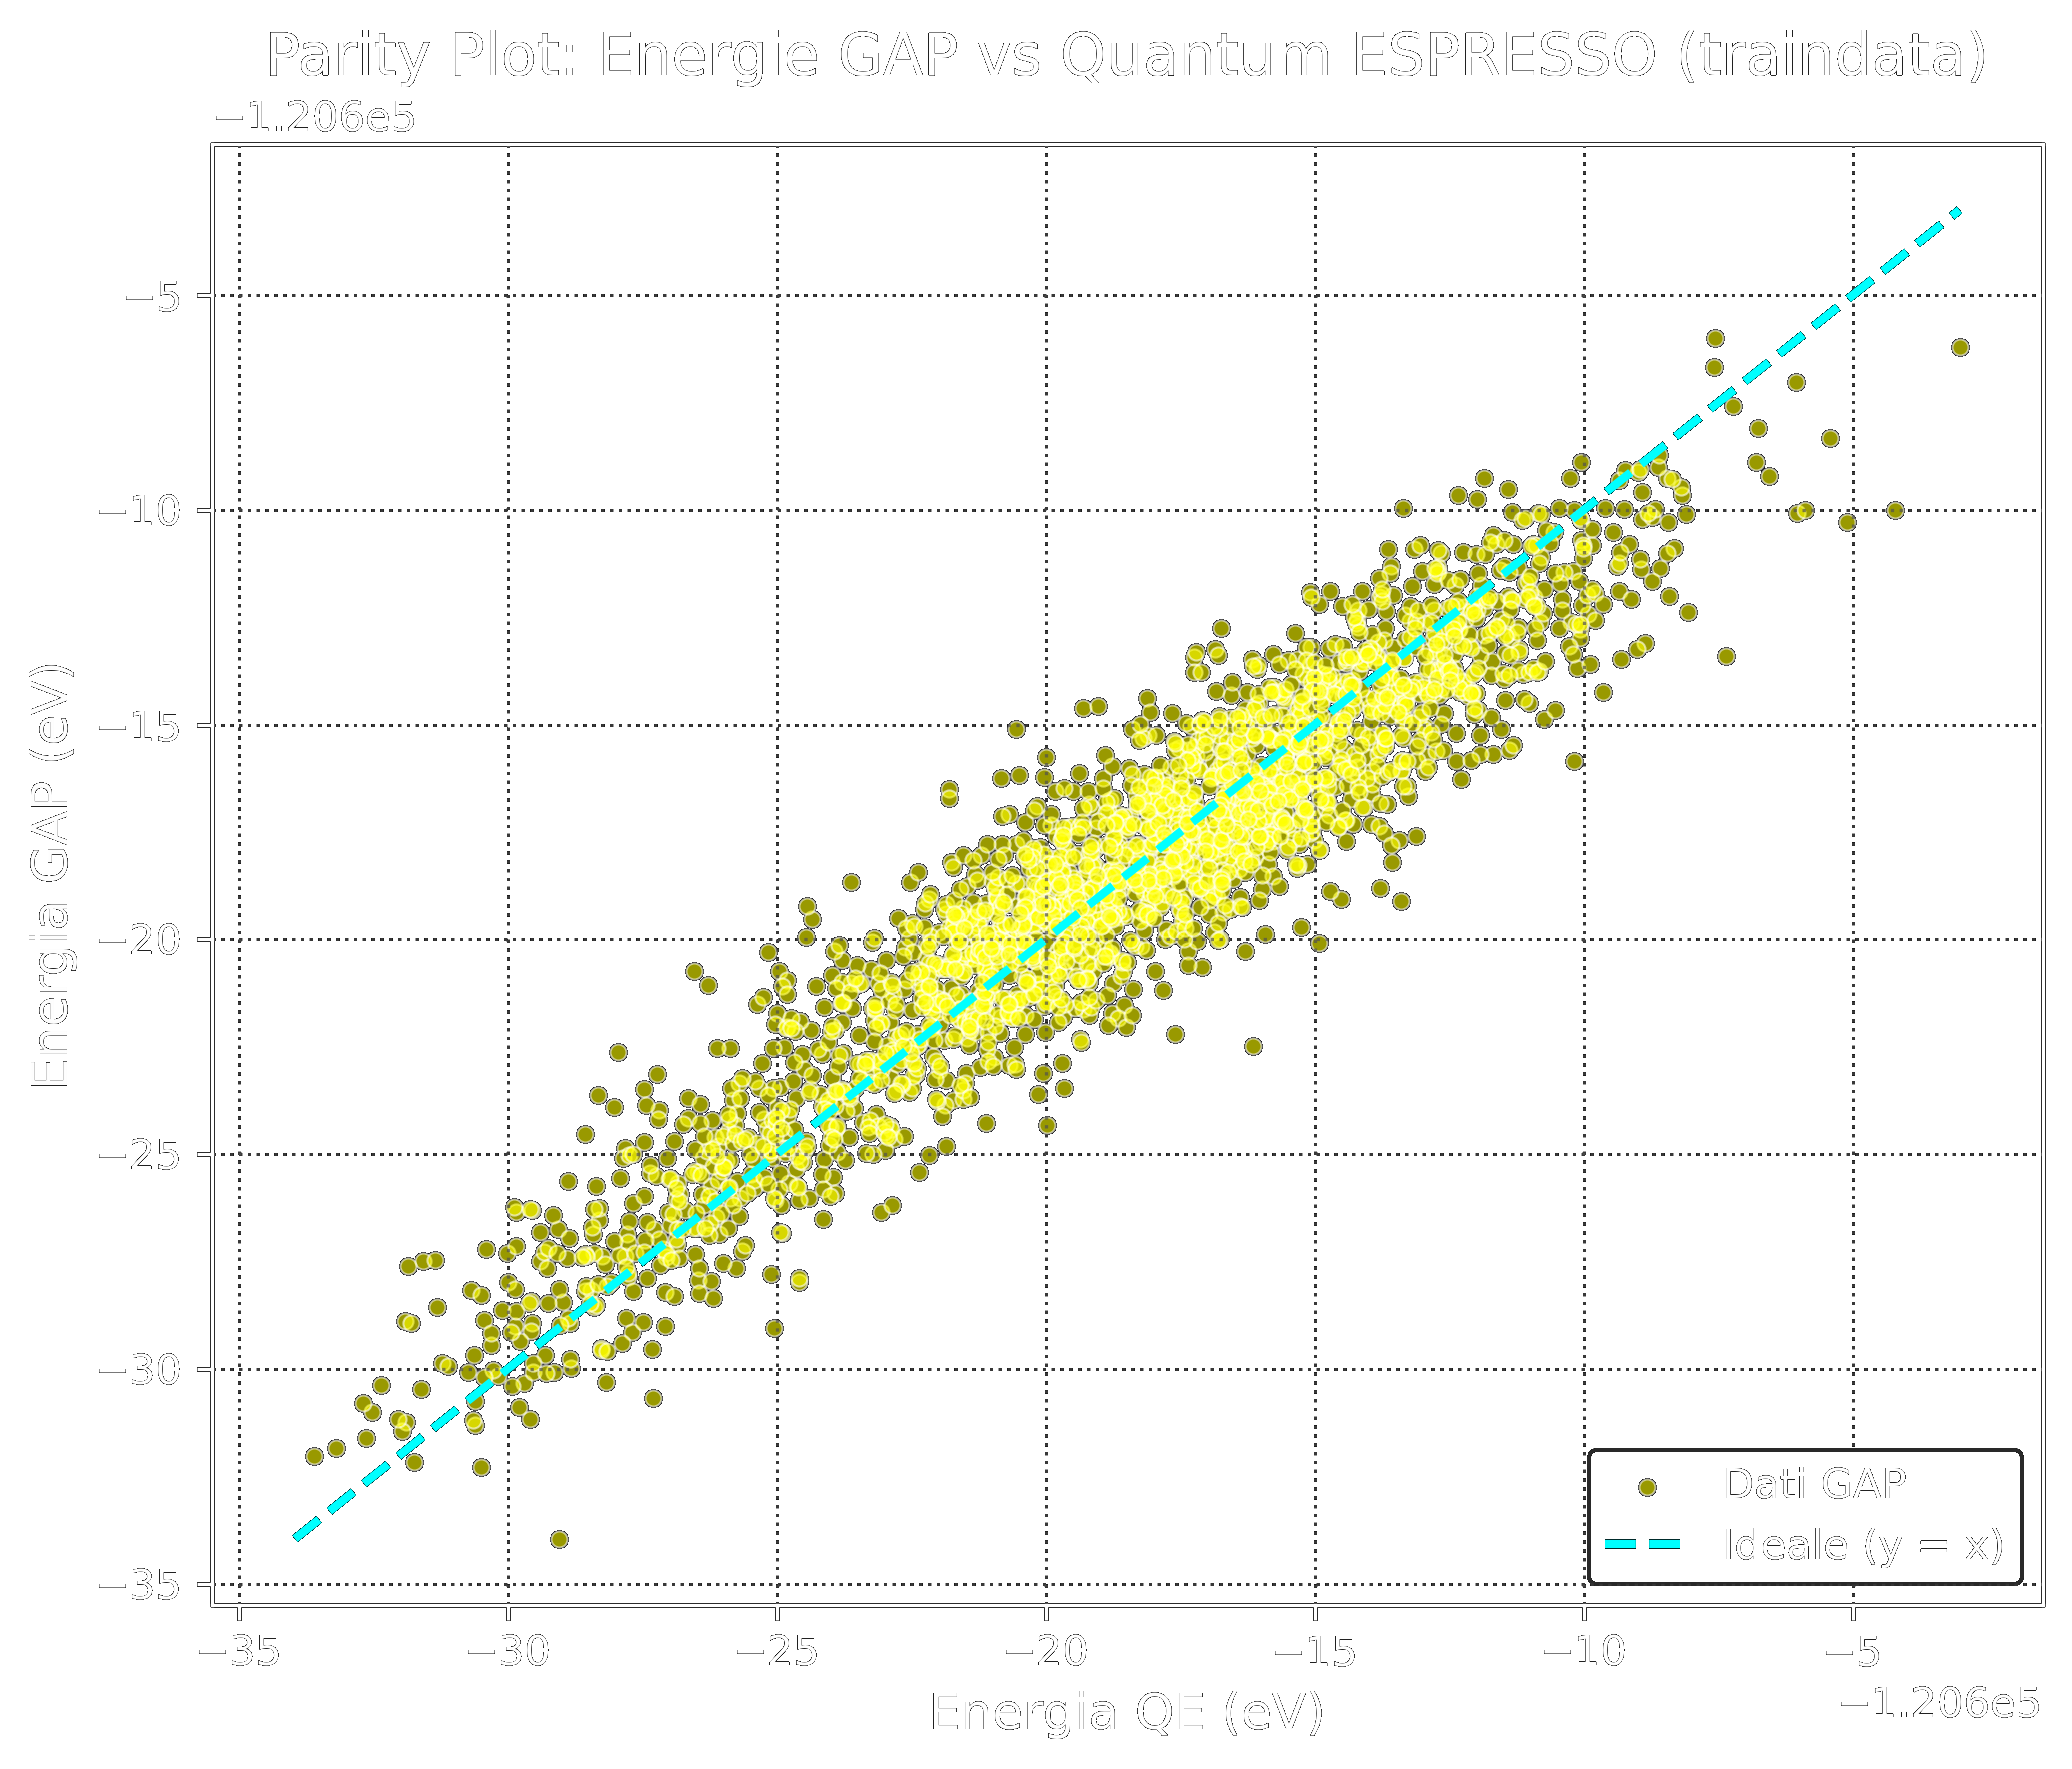
\includegraphics[scale=0.20]{./invnobg/parity_plot_gap_vs_qe-traindata.png}
            \vspace{20pt}
            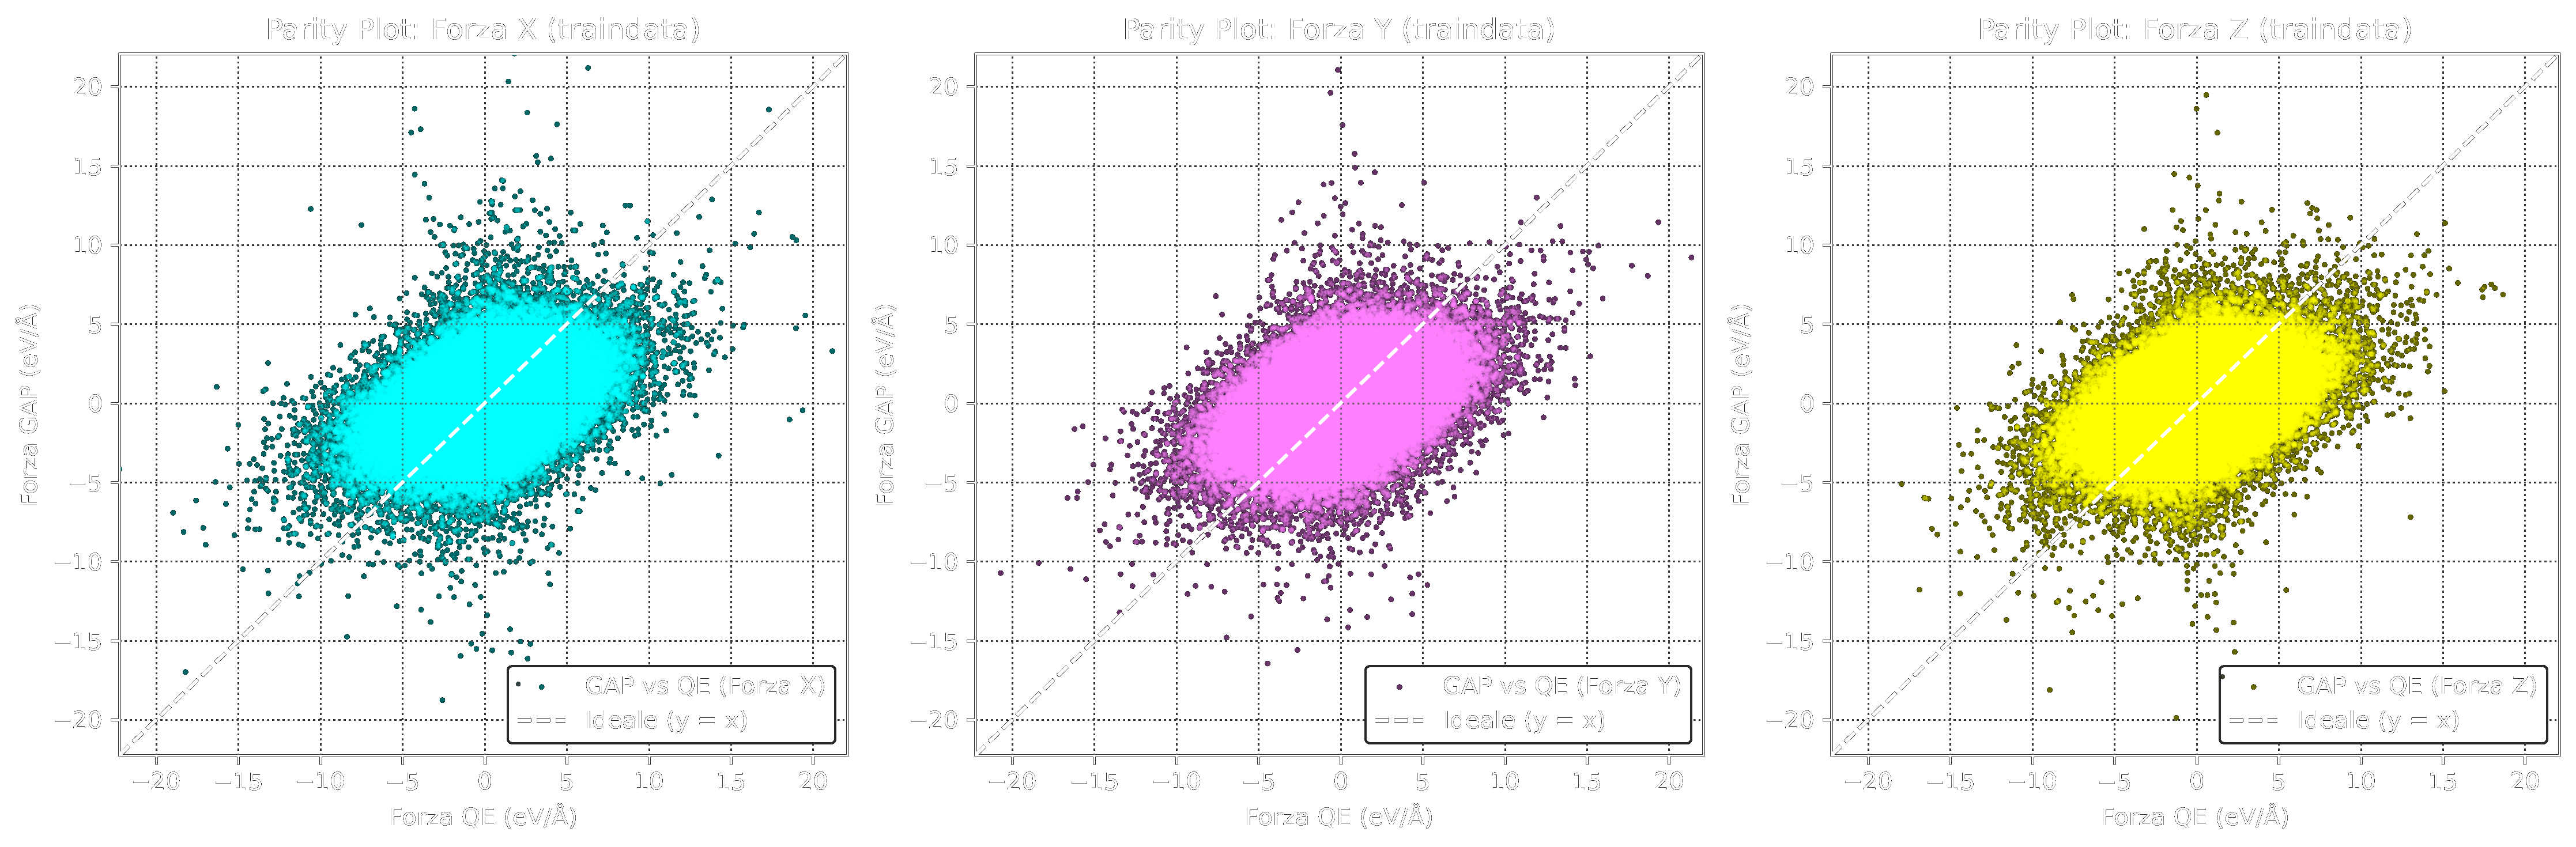
\includegraphics[scale=0.16]{./invnobg/parity_plot_forze-traindata.png}
        
        \end{column}
        % Colonna Destra: Due immagini incolonnate
        \begin{column}{0.46\textwidth}
            
            \centering
            
            Test set
            \vspace{6pt}
            
            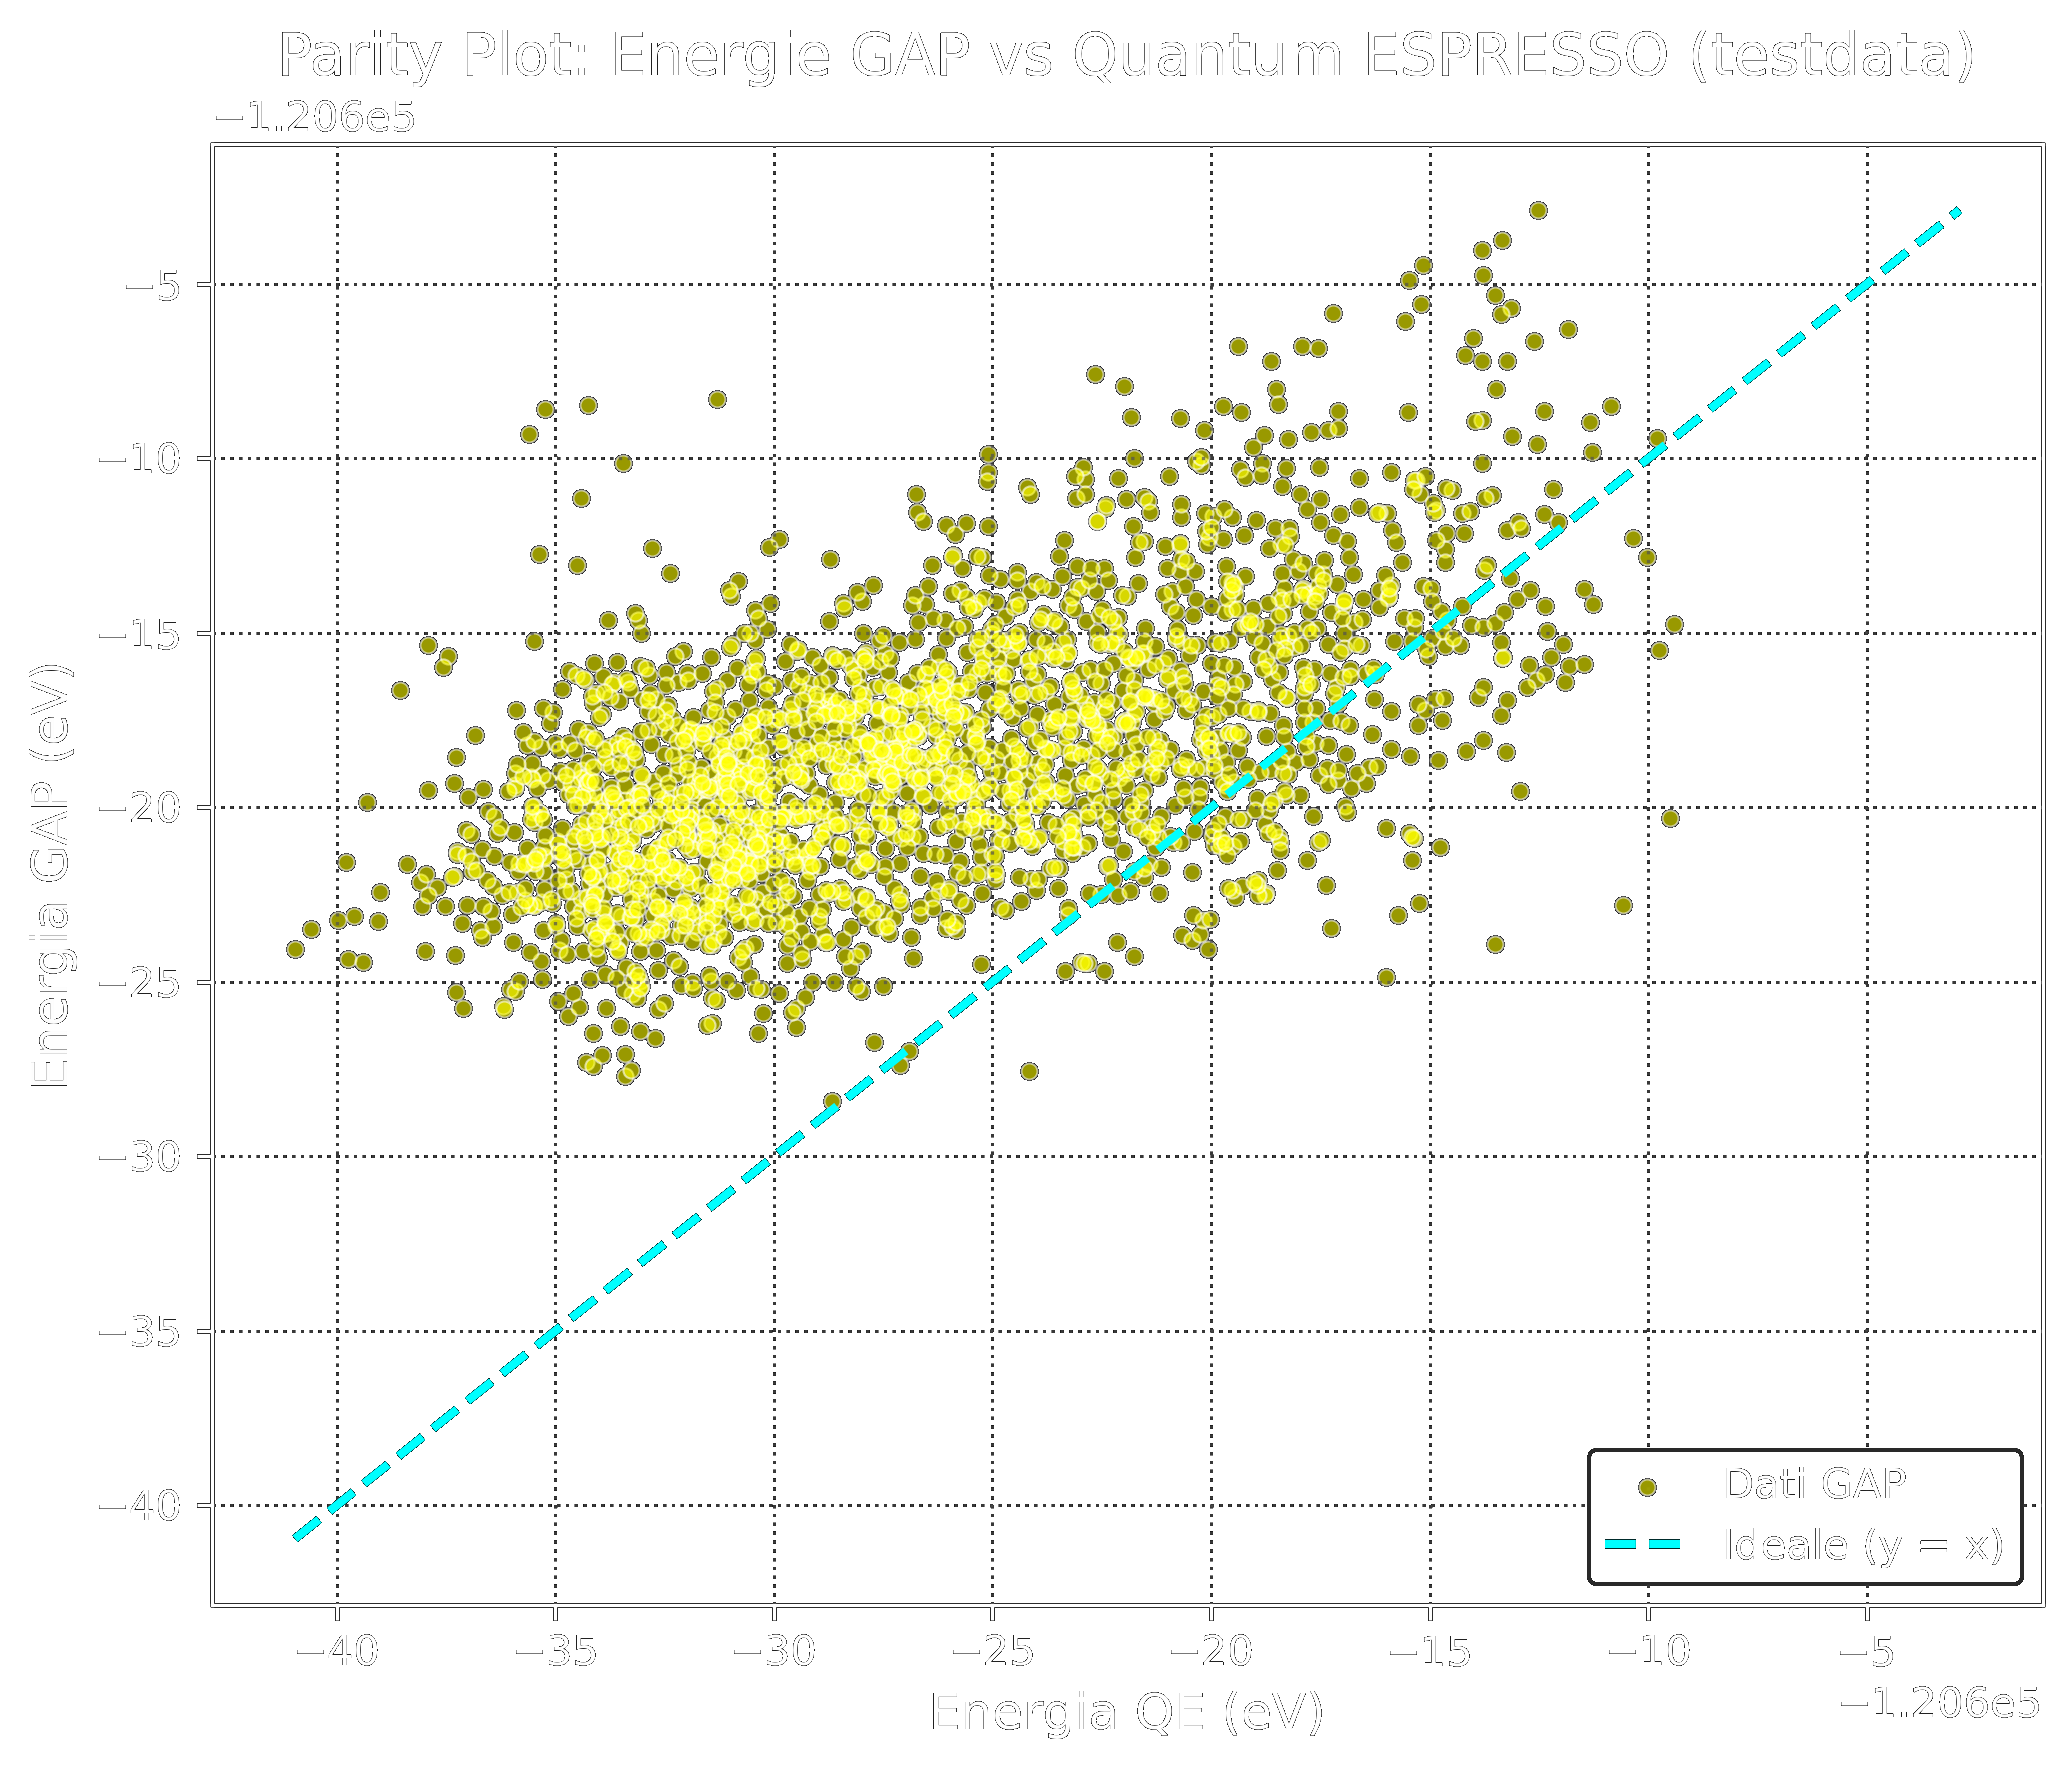
\includegraphics[scale=0.20]{./invnobg/parity_plot_gap_vs_qe-testdata.png}
            \vspace{20pt}
            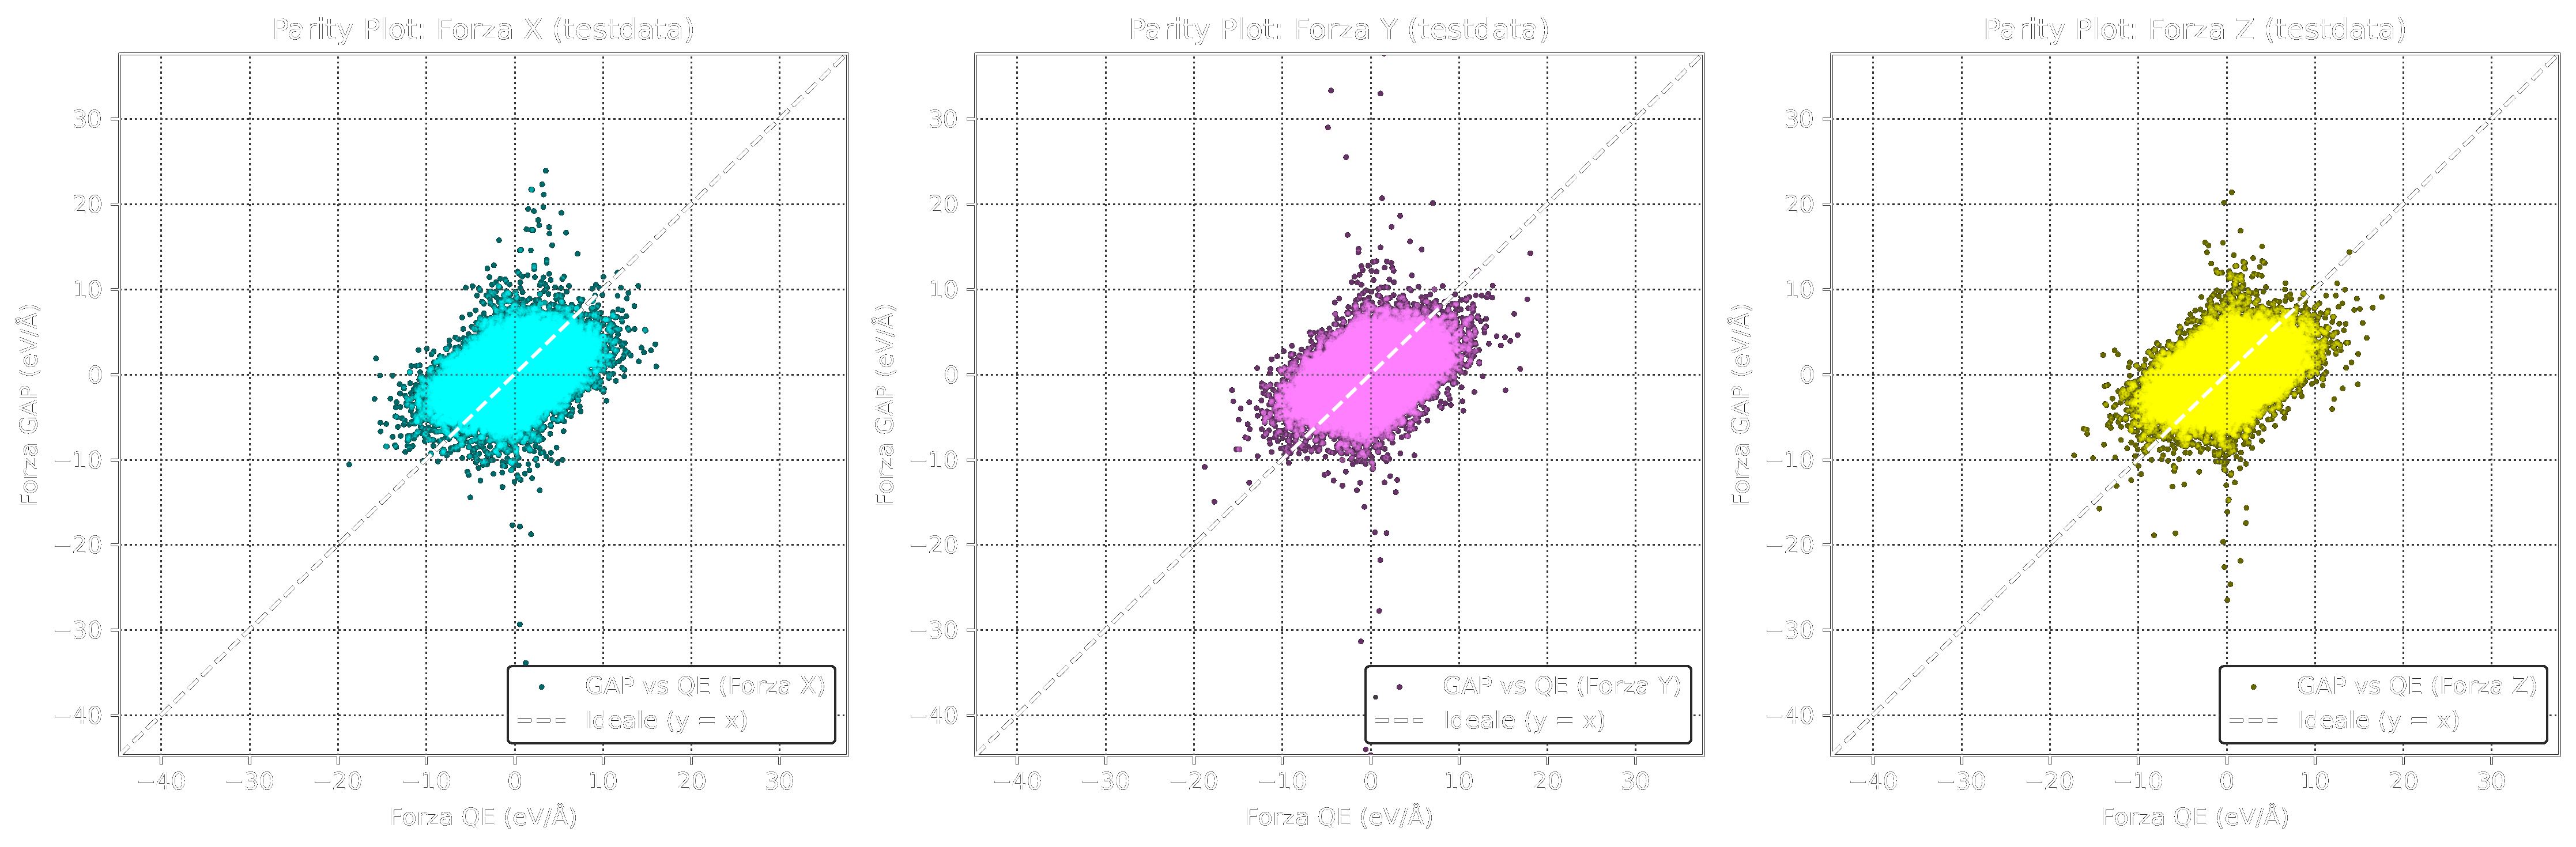
\includegraphics[scale=0.16]{./invnobg/parity_plot_forze-testdata.png}
            
        \end{column}
    \end{columns}
\end{frame}


